\documentclass[aspectratio=169]{beamer}

\usepackage[utf8]{inputenc}
\usepackage[T1]{fontenc}
\usepackage{amsmath}
\usepackage{braket} % quantum notation
\usepackage{tcolorbox} % customization of boxes

\usepackage{tikz}
\usetikzlibrary{tikzmark,positioning,automata}
\usetikzlibrary{shapes.geometric}
\tikzstyle{every picture}+=[remember picture]


\usetheme{CambridgeUS}
\usecolortheme{rose}

\ProvidesPackage{mymacros}[2011/02/23 v1.0 My own macros]

% These options will be applied to all `tcolorboxes`
\tcbset{%
    noparskip,
    colback=gray!10, %background color of the box
    colframe=gray!40, %color of frame and title background
    coltext=black, %color of body text
    coltitle=black, %color of title text 
    fonttitle=\bfseries,
    alerted/.style={coltitle=black, 
                     colframe=blue!70},
    example/.style={coltitle=black, 
                     colframe=blue!90},
    }
%%%%%%%%%%%%%%%%%%


\newif\ifshowtoc
\showtoctrue
\AtBeginSection{%
\ifshowtoc
{\setbeamercolor{background canvas}{bg=red!60}
\begin{frame}[plain]
\frametitle{Outline}
\tableofcontents[currentsection, sectionstyle=show/hide]
\end{frame}}
\fi
}


\title{tbd}
\subtitle{tbd}

\date[tbd]{tbd}
\author[jmaunon]{tbd}
\newcount\colveccount
\newcommand*\colvec[1]{
        \global\colveccount#1
        \begin{pmatrix}
        \colvecnext
}
\def\colvecnext#1{
        #1
        \global\advance\colveccount-1
        \ifnum\colveccount>0
                \\
                \expandafter\colvecnext
        \else
                \end{pmatrix}
        \fi
}


%%%%%%%%%%%%% TIKZ

\tikzset{
	invisible/.style={opacity=0,text opacity=0},
	visible on/.style={alt=#1{}{invisible}},
	alt/.code args={<#1>#2#3}{%
		\alt<#1>{\pgfkeysalso{#2}}{\pgfkeysalso{#3}} 
	},
}

\tikzset{
	background fill/.style={fill=#1},
	background fill/.default={white},
	fill on/.style={alt=#1{}{background fill}},
}

\tikzset{
	background draw/.style={draw=#1},
	background draw/.default={white},
	draw on/.style={alt=#1{}{background draw}},
}

\tikzset{
	background filldraw/.style 2 args={draw=#1, fill=#2},
	background filldraw/.default={white}{white},
	filldraw on/.style={alt=#1{}{background filldraw}},
}

\tikzset{
	background shade/.style={#1},
	background shade/.default={top color=white, bottom color=white},
	shade on/.style={alt=#1{}{background shade}},
}

\tikzset{
	background shadedraw/.style 2 args={draw=#1, #2},
	background shadedraw/.default={white}{top color=white, bottom color=white},
	shadedraw on/.style={alt=#1{}{background shadedraw}},
}

\tikzset{onslide/.code args={<#1>#2}{%
		\only<#1>{\pgfkeysalso{#2}}
	}}


% These options will be applied to all `tcolorboxes`
\tcbset{%
    noparskip,
    colback=gray!10, %background color of the box
    colframe=gray!40, %color of frame and title background
    coltext=black, %color of body text
    coltitle=black, %color of title text 
    fonttitle=\bfseries,
    alerted/.style={coltitle=black, 
                     colframe=blue!70},
    example/.style={coltitle=black, 
                     colframe=blue!90},
    }

%===== custom toc =====
\setbeamertemplate{section in toc}{%
	{\color{orange!70!black}\inserttocsectionnumber.}~\inserttocsection}
\setbeamercolor{subsection in toc}{bg=white,fg=structure}
\setbeamertemplate{subsection in toc}{%
	\hspace{1.2em}{\color{orange}\inserttocsectionnumber.\inserttocsubsectionnumber.}~\inserttocsubsection\par}

%===== custom toc at begin section/subsection =====
\newif\ifshowtoc
\showtoctrue
\AtBeginSection{%
\ifshowtoc
{\setbeamercolor{background canvas}{bg=white}
\begin{frame}[plain]
\frametitle{Outline}

\tableofcontents[currentsection]
\end{frame}}
\fi
}

\newif\ifshowtoc
\showtoctrue
\AtBeginSubsection{%
	\ifshowtoc
	{\setbeamercolor{background canvas}{bg=white}
		\begin{frame}[plain]
			\frametitle{Outline}
						
			\tableofcontents[ currentsection,
			currentsubsection,
			subsectionstyle=show/shaded]
	\end{frame}}
	\fi
}

%===== custom headline =====

\setbeamertemplate{headline}{%

	\begin{beamercolorbox}[ht=2.5ex]{section in head/foot}
		%\vskip2pt\insertnavigation{\paperwidth}\vskip2pt
		\vskip2pt\insertsectionnavigationhorizontal{\paperwidth}{}{\hskip0pt plus1filll}
	\end{beamercolorbox}%
	%   \ifbeamer@theme@subsection%

	\begin{beamercolorbox}[ht=2.5ex,dp=1.125ex,%
		leftskip=.3cm,rightskip=.3cm plus1fil]{subsection in head/foot}
		\vskip2pt\insertsubsectionnavigationhorizontal{\paperwidth}{}{\hskip0pt plus1filll}
	\end{beamercolorbox}%

}

\begin{document}



\begin{frame}
\titlepage
\end{frame}


\begin{frame}[plain]
\frametitle{Outline}
\tableofcontents

\end{frame}

\begin{frame}
\frametitle{Definiciones básicas}

\begin{block}[Producto tensorial]
  Dado $A\in\mathbb{C}^{m\times n}$, $B\in\mathbb{C}^{p\times q}$, el producto tensorial $A\otimes B$ es la matriz            $D\in\mathbb{C}^{pm\times nq}$ tal que:
	\[
		D:=A\otimes B = 		
		\begin{pmatrix}
    a_{11}B & \cdots & a_{1n}B \\
    a_{21}B & \cdots & a_{2n}B \\
    \vdots  &        &  \vdots \\
    a_{m1}B & \cdots & a_{mn}B
  		\end{pmatrix}
	\]
\end{block}


  $x\otimes y = \colvec{2}{1}{0}\otimes\colvec{2}{0}{1}=\colvec{4}{0}{1}{0}{0}$

\end{frame}


\begin{frame}
	\frametitle{Initialization}
	\begin{tikzpicture}[
	expl/.style={draw=black, thick=2pt,fill=blue!20,rounded corners},
	arrow/.style={red!80!black,ultra thick,->,>=latex}]	
	\node[anchor=south west,inner sep=0] (image) at (0,0) {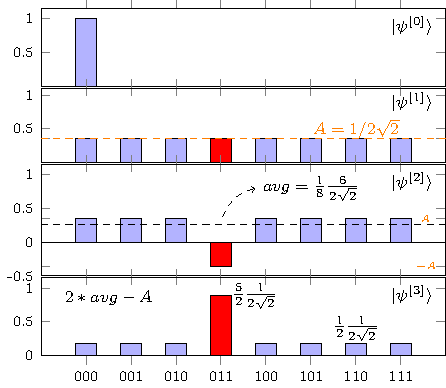
\includegraphics[width=0.5\textwidth]{figures/bar-graph/probs.pdf}};
	\begin{scope}[x={(image.south east)},y={(image.north west)}]
	%\draw[help lines,xstep=.1,ystep=.1] (0,0) grid (1,1);
	%\foreach \x in {0,1,...,9} { \node [anchor=north] at (\x/10,0) {0.\x}; }
	%\foreach \y in {0,1,...,9} { \node [anchor=east] at (0,\y/10) {0.\y}; }
	\node[expl](A) at (1.5,0.875) {\Large Initial state $\ket{\psi^{[0]}}$};
	\node[expl](B) at (1.5,0.65) {\Large Initialization $\ket{\psi^{[1]}}$};
	\node[expl](C) at (1.5,0.4) {\Large Sign flip $\ket{\psi^{[2]}}$};
	\node[expl](D) at (1.5,0.15) {\Large Inversion about average $\ket{\psi^{[3]}}$};
	
	\draw[arrow] (A.south) -- node [right]{Hadamard $H$} (B.north);
	\draw[arrow] (B.south) -- node [right]{Oracle $U_f$} (C.north);
	\draw[arrow] (C.south) -- node [right]{Difussion $U_d$} (D.north);
	\draw[thick,dashed] (0.01,0.575) rectangle (1.85,1);
	\draw[arrow] (D.north east) to[bend right] node [right]{$\frac{\pi}{4}\sqrt{n}$} (B.east);
	\end{scope}
	
	\end{tikzpicture}	
\end{frame}
\begin{frame}
\frametitle{Initialization}
We find a method (unitary operator) to have all the states with the same probability (\textit{principle of superposition}). 
\pause
\begin{eqnarray}
(I^{\otimes n}\otimes X)\left.|0\right\rangle _{n+1}&=&\left.|0\right\rangle _{n}\otimes\left.|1\right\rangle \nonumber\\
H^{\otimes\left(n+1\right)}\left[(I^{\otimes n}\otimes X)\left.|0\right\rangle _{n+1}\right]&=&H^{\otimes n}\left.|0\right\rangle _{n}\otimes H\left.|1\right\rangle \nonumber\\
&=&\sum_{j\in\{0,1\}^{n}}\frac{1}{\sqrt{2^{n}}}\left.|j\right\rangle _{n}\otimes\frac{1}{\sqrt{2}}\left(\left.|0\right\rangle -\left.|1\right\rangle \right)\nonumber\\
&=&\sum_{j\in\{0,1\}^{n}}\alpha_{j}\left.|j\right\rangle _{n}\otimes\frac{1}{\sqrt{2}}\left(\left.|0\right\rangle -\left.|1\right\rangle \right)\nonumber\\
&=&\ket{\psi^{[1]}}\nonumber
\end{eqnarray}
\end{frame}

\begin{frame}
\frametitle{Initialization}

\begin{exampleblock}{3-qubit example: Set ancillary qubit to $\ket{1}$}
\begin{eqnarray}
(I^{\otimes3}\otimes X)\left.|0\right\rangle _{3+1}&=&I^{\otimes3}\left.|0\right\rangle _{3}\otimes X\left.|0\right\rangle \nonumber\\
&=&\begin{pmatrix*}[c]
1&0&0&0&0&0&0&0\\
0&1&0&0&0&0&0&0\\
0&0&1&0&0&0&0&0\\
0&0&0&1&0&0&0&0\\
0&0&0&0&1&0&0&0\\
0&0&0&0&0&1&0&0\\
0&0&0&0&0&0&1&0\\
0&0&0&0&0&0&0&1\\
\end{pmatrix*}\left(\begin{array}{c}
1\\
0\\
0\\
0\\
0\\
0\\
0\\
0
\end{array}\right)\otimes\left(\begin{array}{cc}
0 & 1\\
1 & 0
\end{array}\right)\left(\begin{array}{c}
1\\
0
\end{array}\right)\nonumber\\
&=&\left.|0\right\rangle_3 \otimes\left.|1\right\rangle \nonumber
\end{eqnarray}
\end{exampleblock}


\end{frame}

\begin{frame}
\frametitle{Initialization}
\begin{exampleblock}{3-qubit example: Apply Hadamard gate}
\begin{eqnarray}
\ket{\psi^{[1]}}&=&H^{\otimes\left(3+1\right)}\left[(I^{\otimes3}\otimes X)\left.|0\right\rangle _{n+1}\right]\nonumber\\
&=&H^{\otimes3}\left.|0\right\rangle_3 \otimes H\left.|1\right\rangle\nonumber\\
&=&\frac{1}{\sqrt{2^{3}}}\begin{pmatrix*}[r]
1 & 1 & 1 & 1 & 1 & 1 & 1 & 1\\
1 & -1 & 1 & -1 & 1 & -1 & 1 & -1\\
1 & 1 & -1 & -1 & 1 & 1 & -1 & -1\\
1 & -1 & -1 & 1 & 1 & -1 & -1 & 1\\
1 & 1 & 1 & 1 & -1 & -1 & -1 & -1\\
1 & -1 & 1 & -1 & -1 & 1 & -1 & 1\\
1 & 1 & -1 & -1 & -1 & -1 & 1 & 1\\
1 & -1 & -1 & 1 & -1 & 1 & 1 & -1
\end{pmatrix*}\left(\begin{array}{c}
1\\
0\\
0\\
0\\
0\\
0\\
0\\
0
\end{array}\right)\otimes\frac{1}{\sqrt{2}}\left(\begin{array}{cc}
1 & 1\\
1 & -1
\end{array}\right)\left(\begin{array}{c}
0\\
1
\end{array}\right)\nonumber
\end{eqnarray}
\end{exampleblock}
\end{frame}

\begin{frame}
	\frametitle{Initialization}
	\begin{exampleblock}{3-qubit example: Apply Hadamard gate}
		\begin{eqnarray}
			\ket{\psi^{[1]} }&=&\frac{1}{\sqrt{2^{3}}}\begin{pmatrix*}
			1 1 1 1 1 1 1 1
			\end{pmatrix*}^{\dagger}\otimes\frac{1}{\sqrt{2}}\left(\begin{array}{c}
			1\\
			-1
			\end{array}\right)\nonumber\\
			&=&[ \frac{1}{2\sqrt{2}}\left.|000\right\rangle +\frac{1}{2\sqrt{2}}\left.|001\right\rangle +\frac{1}{2\sqrt{2}}\left.|010\right\rangle +\frac{1}{2\sqrt{2}}\left.|011\right\rangle \nonumber\\
			&+&\frac{1}{2\sqrt{2}}\left.|100\right\rangle +\frac{1}{2\sqrt{2}}\left.|101\right\rangle +\frac{1}{2\sqrt{2}}\left.|110\right\rangle +\frac{1}{2\sqrt{2}}\left.|111\right\rangle] \nonumber\\
			&\otimes&\frac{1}{\sqrt{2}}\left(\left.|0\right\rangle -\left.|1\right\rangle \right)		\nonumber	
		\end{eqnarray}
	\end{exampleblock}
\end{frame}

\begin{frame}{}
	\frametitle{Initialization}
	\begin{exampleblock}{3-qubit example: Summary}
		\begin{eqnarray}
			\ket{\psi^{[1]} }&=&
			H^{\otimes\left(3+1\right)}\left[(I^{\otimes3}\otimes X)\left.|0\right\rangle _{n+1}\right]\nonumber\\
			&=&[\frac{1}{2\sqrt{2}}\left.|000\right\rangle +\frac{1}{2\sqrt{2}}\left.|001\right\rangle +\frac{1}{2\sqrt{2}}\left.|010\right\rangle +\frac{1}{2\sqrt{2}}\left.|011\right\rangle\nonumber\\ &+&\frac{1}{2\sqrt{2}}\left.|100\right\rangle +\frac{1}{2\sqrt{2}}\left.|101\right\rangle +\frac{1}{2\sqrt{2}}\left.|110\right\rangle +\frac{1}{2\sqrt{2}}\left.|111\right\rangle ]\nonumber\\
			&\otimes&\frac{1}{\sqrt{2}}\left(\left.|0\right\rangle -\left.|1\right\rangle \right)\nonumber\\
			&=&\sum_{j\in\{0,1\}^{n}}\frac{1}{\sqrt{2^{n}}}\left.|j\right\rangle _{n}\otimes\frac{1}{\sqrt{2}}\left(\left.|0\right\rangle -\left.|1\right\rangle \right)=\ket{\psi^{[1]} }\nonumber
		\end{eqnarray}
	\end{exampleblock}
\end{frame}



\begin{frame}
	\frametitle{Sign flip}
	\begin{tikzpicture}[
	expl/.style={draw=black, thick=2pt,fill=blue!20,rounded corners},
	arrow/.style={red!80!black,ultra thick,->,>=latex}]	
	\node[anchor=south west,inner sep=0] (image) at (0,0) {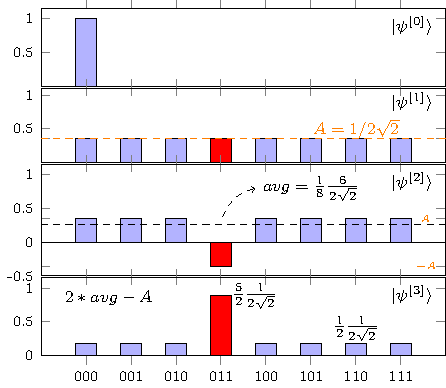
\includegraphics[width=0.5\textwidth]{figures/bar-graph/probs.pdf}};
	\begin{scope}[x={(image.south east)},y={(image.north west)}]
	%\draw[help lines,xstep=.1,ystep=.1] (0,0) grid (1,1);
	%\foreach \x in {0,1,...,9} { \node [anchor=north] at (\x/10,0) {0.\x}; }
	%\foreach \y in {0,1,...,9} { \node [anchor=east] at (0,\y/10) {0.\y}; }
	\node[expl](A) at (1.5,0.875) {\Large Initial state $\ket{\psi^{[0]}}$};
	\node[expl](B) at (1.5,0.65) {\Large Initialization $\ket{\psi^{[1]}}$};
	\node[expl](C) at (1.5,0.4) {\Large Sign flip $\ket{\psi^{[2]}}$};
	\node[expl](D) at (1.5,0.15) {\Large Inversion about average $\ket{\psi^{[3]}}$};
	
	\draw[arrow] (A.south) -- node [right]{Hadamard $H$} (B.north);
	\draw[arrow] (B.south) -- node [right]{Oracle $U_f$} (C.north);
	\draw[arrow] (C.south) -- node [right]{Difussion $U_d$} (D.north);
	\draw[thick,dashed] (0.01,0.3) rectangle (1.85,0.75);
	\draw[arrow] (D.north east) to[bend right] node [right]{$\frac{\pi}{4}\sqrt{n}$} (B.east);
	\end{scope}	
	\end{tikzpicture}	
\end{frame}
\begin{frame}
	\frametitle{Sign flip}
	We find a method (unitary operator) which flip the sign of the state of interest.
	\pause
	\begin{block}{\textit{Quantum Oracle}}
		It is defined the operator $U_f$: 
		\[U_{f}:\left.|j\right\rangle _{n}\otimes\left.|y\right\rangle _{1}\rightarrow\left.|j\right\rangle _{n}\otimes\left.|y\oplus f\left(j\right)\right\rangle _{1},\]
		where $\oplus$ is the sum operator in mod 2, and $f\left(j\right)=\left\{ \begin{array}{cc}
		1  & j=l\\
		0  & j\neq l
		\end{array}\right\} $
	\end{block}
	
	
	\begin{center}
		\begin{tabular}{|c c |c|} 
			\hline
			A & B & XOR \\ 
			\hline\hline
			0&0&0  \\ 
			\hline
			0&1&1  \\ 
			\hline
			1&0&1  \\
			\hline
			1&1&0 \\
			\hline
		\end{tabular}
	\end{center}
\end{frame}

\begin{frame}
	\frametitle{Sign flip}
	We apply $U_f$ (\textit{Quantum Oracle}) to the previous state $\psi^{[1]}$
	\begin{eqnarray}
		\ket{\psi^{[2]}}&=& U_{f}\ket{\psi^{[1]}}\nonumber\\
			&=&U_{f}\left(\sum_{j\in\{0,1\}^{n}}\alpha_{j}\left.|j\right\rangle _{n}\otimes\frac{1}{\sqrt{2}}\left(\left.|0\right\rangle -\left.|1\right\rangle \right)\right)\nonumber\\
		&=&U_{f}\left(\alpha_{l}\left.|l\right\rangle _{n}\otimes\frac{1}{\sqrt{2}}\left(\left.|0\right\rangle -\left.|1\right\rangle \right)+\sum_{
			j\in\{0,1\}^{n};\;
			j\neq l
			}\alpha_{j}\left.|j\right\rangle _{n}\otimes\frac{1}{\sqrt{2}}\left(\left.|0\right\rangle -\left.|1\right\rangle \right)\right)\nonumber\\
		&=&\left(\tikz[baseline]{
			\node[fill=blue!20,anchor=base, fill on=<2->,draw=red,rounded corners,draw on =<3>] (A)
			{$ -\alpha_{l}\left.|l\right\rangle _{n}$};
		} 
				 +\sum_{j\in\{0,1\}^{n};\;
				 	j\neq l}\alpha_{j}\left.|j\right\rangle _{n}\right)\otimes\tikz[baseline]{
			\node[fill=blue!20,anchor=base, fill on=<3>,draw=red,draw on =<3>,rounded corners] (AA)
			{$ \frac{1}{\sqrt{2}}\left(\left.|0\right\rangle -\left.|1\right\rangle \right)$};\nonumber
		} 
	\end{eqnarray}
	\begin{tikzpicture}[
	remember picture,
	overlay,
	expl/.style={draw=red, thick=2pt,fill=blue!20,rounded corners},
	arrow/.style={red!80!black,ultra thick,->,>=latex}
	]
	\onslide<2->{\node[expl, xshift = -3cm](B) at (current page.center) {\Large sign flip!};}
	\onslide<2->{\draw[arrow]
	(A.north) to[bend left] (B.south);}
	\onslide<3->{\node[expl, xshift = 3cm](BB) at (current page.center) {\Large Extra qubit!};}
	\onslide<3->{\draw[arrow]
		(AA.north) to[bend right] (BB.south);}
	\end{tikzpicture}
\end{frame}


\begin{frame}
	\frametitle{Sign flip\footnote{This slide shows the result of applying $U_f$ but not how is applied. This is because this step of the algorithm depends on the specific problem.}}
	\begin{exampleblock}{3-qubit example: Quantum Oracle}
		\begin{eqnarray}		
		\ket{\psi^{[2]}} &=& U_f\ket{\psi^{[1]}} \nonumber\\
		&=&[\frac{1}{2\sqrt{2}}\left.|000\right\rangle +\frac{1}{2\sqrt{2}}\left.|001\right\rangle +\frac{1}{2\sqrt{2}}\left.|010\right\rangle -\frac{1}{2\sqrt{2}}\left.|011\right\rangle\nonumber\\ &+&\frac{1}{2\sqrt{2}}\left.|100\right\rangle +\frac{1}{2\sqrt{2}}\left.|101\right\rangle +\frac{1}{2\sqrt{2}}\left.|110\right\rangle +\frac{1}{2\sqrt{2}}\left.|111\right\rangle ]\nonumber\\
		&\otimes&\frac{1}{\sqrt{2}}\left(\left.|0\right\rangle -\left.|1\right\rangle \right)\nonumber
		\end{eqnarray}
	\end{exampleblock}
\end{frame}


\end{document}